\documentclass{article}
\title{On the length of mature microRNAs}
\author{Dave Tang  \\
	RIKEN Yokohama \\
	\and 
	Derek de Rie \\
	VU University Amsterdam \\
	}

\date{\today}

\usepackage{graphicx}
\graphicspath{ {image/} }

\usepackage{hyperref}
\hypersetup{
   colorlinks,
   citecolor=black,
   filecolor=black,
   linkcolor=black,
   urlcolor=black
}

\begin{document}

\maketitle

\begin{abstract}
MicroRNAs (miRNAs) blah blah

\end{abstract}

\section{Introduction}

MicroRNAs were discovered in 1993\cite{pmid8252621}.

\section{Methods and results}\label{method_and_result}

All code underlying this work is available at \url{https://github.com/davetang/mirna_length}.

\begin{figure}[h]
   \centering
   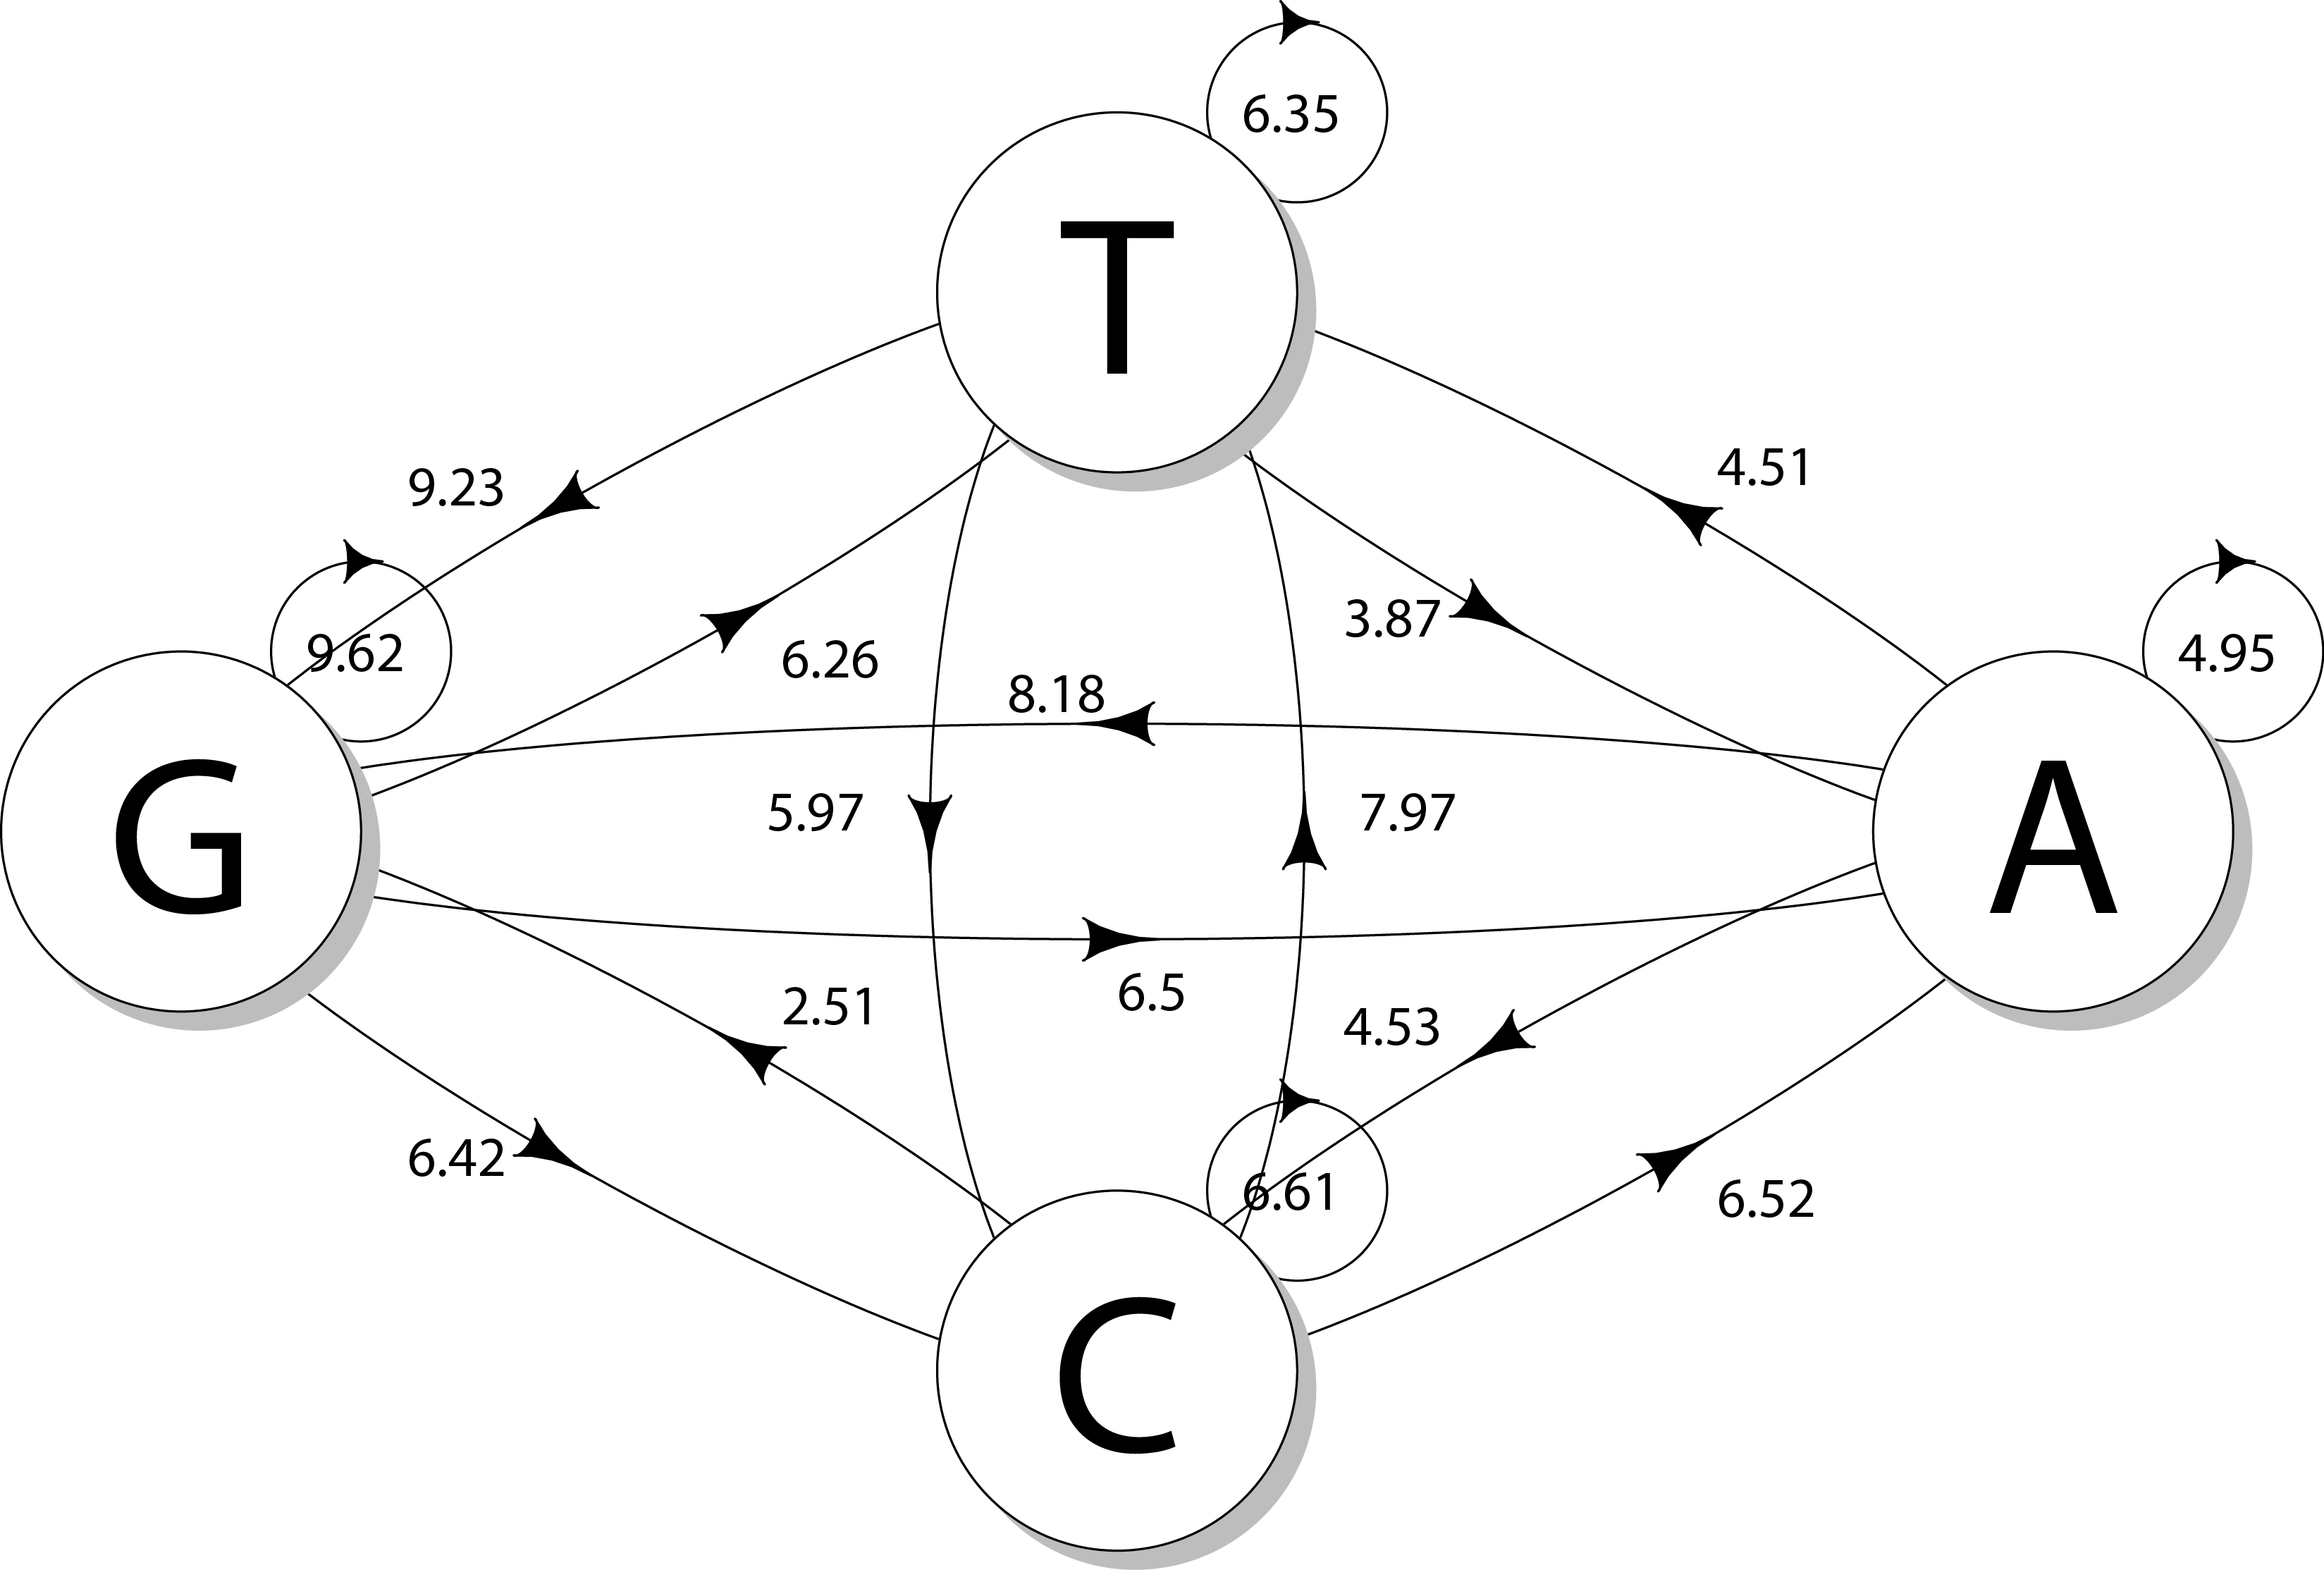
\includegraphics[width=\textwidth,natwidth=3297,natheight=2227]{image/transition.png}
   \caption{Transition diagram based on dinucleotide frequencies of miRBase human miRNAs.}
   \label{fig:transition}
\end{figure}

\section{Discussion}\label{discussion}

\section{Conclusions}\label{conclusion}

\bibliographystyle{unsrt}
\bibliography{ref}

\end{document}
